%! Compiler = XeLaTeX
% !TeX program = xelatex
% !TEX TS-program = xelatex
\documentclass[12pt,a4paper]{article}

\usepackage{iftex}
\ifPDFTeX
  \usepackage[utf8]{inputenc}
  \usepackage[T1]{fontenc}
  \usepackage[english]{babel}
  \babelprovide[import, main]{french}
  \makeatletter
  \providecommand{\xpg@aux}[2]{}
  \makeatother
\else
  \usepackage{fontspec}
  \usepackage{polyglossia}
  \setmainlanguage{french}
\fi

\usepackage[top=2.5cm, bottom=2.5cm, left=2.5cm, right=2.5cm, headheight=14pt]{geometry}
\usepackage{setspace}
\onehalfspacing

\usepackage{microtype}
\usepackage[dvipsnames,table]{xcolor}
\definecolor{primaryblue}{HTML}{8B0000}
\definecolor{lightgray}{HTML}{F5F5F5}
\definecolor{codegray}{HTML}{EEEEEE}
\definecolor{accent}{HTML}{E53935}

\usepackage{graphicx}
\usepackage{booktabs}
\usepackage{array}
\usepackage{tabularx}
\usepackage{longtable}
\usepackage{float}

\usepackage{listings}
\lstdefinestyle{mystyle}{
    backgroundcolor=\color{codegray},
    commentstyle=\color{OliveGreen}\itshape,
    keywordstyle=\color{primaryblue}\bfseries,
    stringstyle=\color{accent},
    numberstyle=\tiny\color{gray},
    basicstyle=\ttfamily\small,
    breakatwhitespace=false,
    breaklines=true,
    captionpos=b,
    keepspaces=true,
    numbers=left,
    numbersep=5pt,
    showspaces=false,
    showstringspaces=false,
    showtabs=false,
    tabsize=2,
    frame=single,
    rulecolor=\color{gray!30},
    framerule=0.5pt,
}
\lstset{style=mystyle}

\usepackage{amsmath}
\usepackage{amssymb}

\usepackage[hidelinks, colorlinks=true, linkcolor=primaryblue, urlcolor=primaryblue, citecolor=primaryblue]{hyperref}

\usepackage{fancyhdr}
\pagestyle{fancy}
\fancyhf{}
\fancyhead[L]{\small\textcolor{gray}{5.3 - Projet}}
\fancyhead[R]{\small\textcolor{gray}{M1 - A - Evan DYNAK}}
\fancyfoot[C]{\thepage}
\renewcommand{\headrulewidth}{0.4pt}

\usepackage{enumitem}
\usepackage{fancybox}
\usepackage{titlesec}

\titleformat{\section}
  {\color{primaryblue}\Large\bfseries}
  {\thesection}{1em}{}[\color{primaryblue}\hrule]

\titleformat{\subsection}
  {\color{primaryblue!80}\large\bfseries}
  {\thesubsection}{1em}{}

\titleformat{\subsubsection}
  {\bfseries\normalsize}
  {\thesubsubsection}{1em}{}

\newenvironment{infobox}[1][]{%
  \par\vspace{6pt}%
  {\color{primaryblue!50}\rule{\linewidth}{1pt}}%
  \nopagebreak\par\nopagebreak%
  \noindent\begin{minipage}{\linewidth}%
  \setlength{\parskip}{4pt}%
  \if\relax\detokenize{#1}\relax\else\textbf{#1}\par\fi%
}{%
  \end{minipage}\par%
  {\color{primaryblue!50}\rule{\linewidth}{1pt}}%
  \par\vspace{6pt}%
}

\newenvironment{warnbox}[1][]{%
  \par\vspace{6pt}%
  {\color{orange!60}\rule{\linewidth}{1pt}}%
  \nopagebreak\par\nopagebreak%
  \noindent\begin{minipage}{\linewidth}%
  \setlength{\parskip}{4pt}%
  \if\relax\detokenize{#1}\relax\else\textbf{#1}\par\fi%
}{%
  \end{minipage}\par%
  {\color{orange!60}\rule{\linewidth}{1pt}}%
  \par\vspace{6pt}%
}

\begin{document}
\begin{titlepage}
    \centering
    \vspace*{2cm}

    {\LARGE\textbf{M1 - Programmation de spécialité (UE5.3)}\par}

    \vspace{2.5cm}

    \rule{\linewidth}{1.5pt}\par
    \vspace{0.4cm}
    {\Huge\bfseries\color{primaryblue} -- Projet -- \\Moteur de Recherche\par}
    \vspace{0.3cm}
    {\large Analyse, conception, architecture découplée\\et étapes de réalisation du projet\par}
    \vspace{0.4cm}
    \rule{\linewidth}{1.5pt}\par

    \vspace{2cm}

    \begin{tabular}{rl}
        \textbf{Auteur :}    	& Evan DYNAK \\[4pt]
        \textbf{Année :}     	& 2026--2027 \\[4pt]
        \textbf{Lien du dépôt:}	& \url{https://github.com/Ashzuu/SearchEngine}
    \end{tabular}

\end{titlepage}

\thispagestyle{empty}
\newpage

\begin{abstract}
Ce rapport rend compte de l'analyse, la conception et la réalisation d'un moteur de recherche, développé dans le cadre de l'UE5.3 de Master 1. Le système extrait des publications textuelles depuis deux sources de données : Reddit et Arxiv, assurant la persistance des données dans un format tabulaire optimisé (format de fichier csv), puis applique une indexation vectorielle basée sur le schéma de pondération TF-IDF et le stockage en matrices. L'interrogation par requête utilisateur repose sur la similarité cosinus. L'application est structurée selon une architecture client-serveur moderne découplée : un back-end en Python (FastAPI) exposant une API REST stricte et un front-end en Angular (version 22) conçu en \textit{Single Page Application}. Ce document retrace en détail la démarche d'architecture, les pistes de réflexion, les algorithmes et les tests.
\end{abstract}

\newpage
\tableofcontents
\newpage

\section{Les spécifications}
\subsection{Contexte et problématique}

L'objectif est de comprendre l'ensemble des processus permettant qu'un moteur de recherche fonctionne. De ce fait, il a été décidé de réaliser un moteur de recherche simpliste sur un domaine de recherche particulier : \textit{Machine Learning}, avec une interface web très légère, dans le but de manipuler les notions mathématiques et la gestion des données. Selon ce contexte, les étapes de réalisation ont été les suivantes :

\begin{itemize}
    \item Récolter des corpus documentaires réels issus du Web à partir d'APIs publiques ;
    \item Modéliser et structurer ces données selon les principes de la programmation orientée objet ;
    \item Représenter mathématiquement le corpus sous forme vectorielle afin de permettre une recherche par pertinence plutôt qu'une simple recherche exacte de motifs ;
    \item Fournir une interface de consultation intuitive pour les utilisateurs finaux.
\end{itemize}

\subsection{Accès au projet}

Le projet est sur Github, sur \href{https://github.com/Ashzuu/SearchEngine}{le même lien} que donné précédemment.

En cas de problématique lié à l'accès du projet, vous pouvez me contacter via le lien suivant : \href{mailto:evan.dynak@univ-lyon2.fr}{Envoyer un mail} (Mail étudiant)

\subsection{Spécifications fonctionnelles}

Le cahier des charges du logiciel définit sept exigences fonctionnelles majeures :

\begin{enumerate}
    \item \textbf{Collecte multi-sources} : Extraire automatiquement des documents à partir d'au moins deux plateformes externes distinctes avec des volumétries représentatives. Pour ce projet, les deux sources ciblées sur la thématique du \textit{Machine Learning} sont :
        \begin{itemize}
            \item L'API Reddit, via le wrapper officiel \texttt{praw}, interrogeant le subreddit spécialisé \texttt{r/MachineLearning} ;
            \item L'API publique d'ArXiv, via le protocole REST/HTTP et l'analyse syntaxique de flux XML (\texttt{xmltodict}).
        \end{itemize}
    \item \textbf{Persistance et mise en cache des données} : Consigner les données collectées dans un fichier structuré (\texttt{data.csv}) avec délimiteur tabulation afin d'assurer \\l'indépendance vis-à-vis du réseau lors des lancements ultérieurs.
    \item \textbf{Prétraitement et nettoyage} : Normaliser la casse, éliminer les caractères parasites, les tabulations, les sauts de ligne et la ponctuation superflue afin d'homogénéiser le texte.
    \item \textbf{Construction de l'index vectoriel} : Établir le vocabulaire global du corpus, calculer les fréquences de termes (\textit{Term Frequency}, TF) et les fréquences de documents (\textit{Document Frequency}, DF), puis synthétiser une matrice TF-IDF.
    \item \textbf{Moteur de recherche par similarité cosinus} : Recevoir une requête utilisateur textuelle, la projeter dans l'espace vectoriel du vocabulaire, calculer la similarité cosinus avec l'ensemble des documents et renvoyer la liste triée des $n$ meilleurs résultats.
    \item \textbf{Concordancier et statistiques lexicales} : Offrir la possibilité d'analyser le contexte immédiat (gauche et droit) d'un motif textuel donné, ainsi que d'extraire la distribution statistique des mots les plus fréquents.
    \item \textbf{Interface graphique interactive} : Proposer une application Web permettant à un utilisateur lambda de saisir sa requête et de visualiser instantanément les métadonnées et extraits des documents trouvés.
\end{enumerate}

\subsection{Spécifications non-fonctionnelles}

\begin{enumerate}
    \item \textbf{Efficacité spatiale et temporelle} : L'indexation vectorielle sur un vocabulaire comprenant des dizaines de milliers de termes ne doit pas saturer la mémoire vive. Le recours à des matrices creuses s'impose.
    \item \textbf{Modularité et patrons de conception} : Le code doit respecter les principes SOLID, en séparant la couche d'accès aux données (\textit{Repository}), la logique métier (\textit{Services}), la représentation (\textit{Models} et \textit{DTOs}) et l'exposition d'API (\textit{Controllers}).
    \item \textbf{Architecture découplée} : Le back-end et le front-end doivent fonctionner en processus indépendants, échangeant exclusivement par HTTP/JSON au moyen d'un contrat d'interface stable.
    \item \textbf{Unicité au démarrage} : Le processus de récupération des données doit vérifier l'état du stockage local afin d'éviter les surcoûts d'appels réseau ou le duplicata des données.
\end{enumerate}

\newpage

\section{L'analyse}

\subsection{Environnement de travail retenu}

\subsubsection{Back-end : Python 3 et FastAPI}

Pour la réalisation du back-end, le langage \textbf{Python 3.14} associé au framework web \textbf{FastAPI} :
\begin{itemize}
    \item \textbf{Langage imposée par le sujet}
    \item \textbf{Utilisation de FastAPI}: Le choix de cette bibliothèque est liée au fait qu'elle apporte tous les éléments nécessaires pour la création d'une API simple et rapide, permettant de ne pas avoir à recréer ceux-ci.
\end{itemize}

\subsubsection{Front-end : Angular}
Pour la réalisation du front-end, le langage \textbf{TypeScript} associé au framework web \textbf{Angular v22}
\begin{itemize}
	\item \textbf{Modularité des composants et des fonctionnalités} : Angular propose une modulation très forte des fonctionnalités et dépendances grâce aux injections de dépendances intégrées au framework.
	\item \textbf{Facilité de maintenance} : La simplicité de la maintenance d'Angular permet de limiter la dette technique des applications développées.
	\item \textbf{Rapidité} : Angular réalise des applications qui peuvent être soit côté client, soit côté serveur : dans ce projet, il a été choisi d'utiliser le mode "côté client" car cela permet d'avoir des meilleures performances : en effet, tous les calculs sont faits via le serveur Python, de ce fait il n'est pas nécessaire d'avoir également des calculs pour le front côté serveur.
\end{itemize}

\subsection{Architecture de classes}

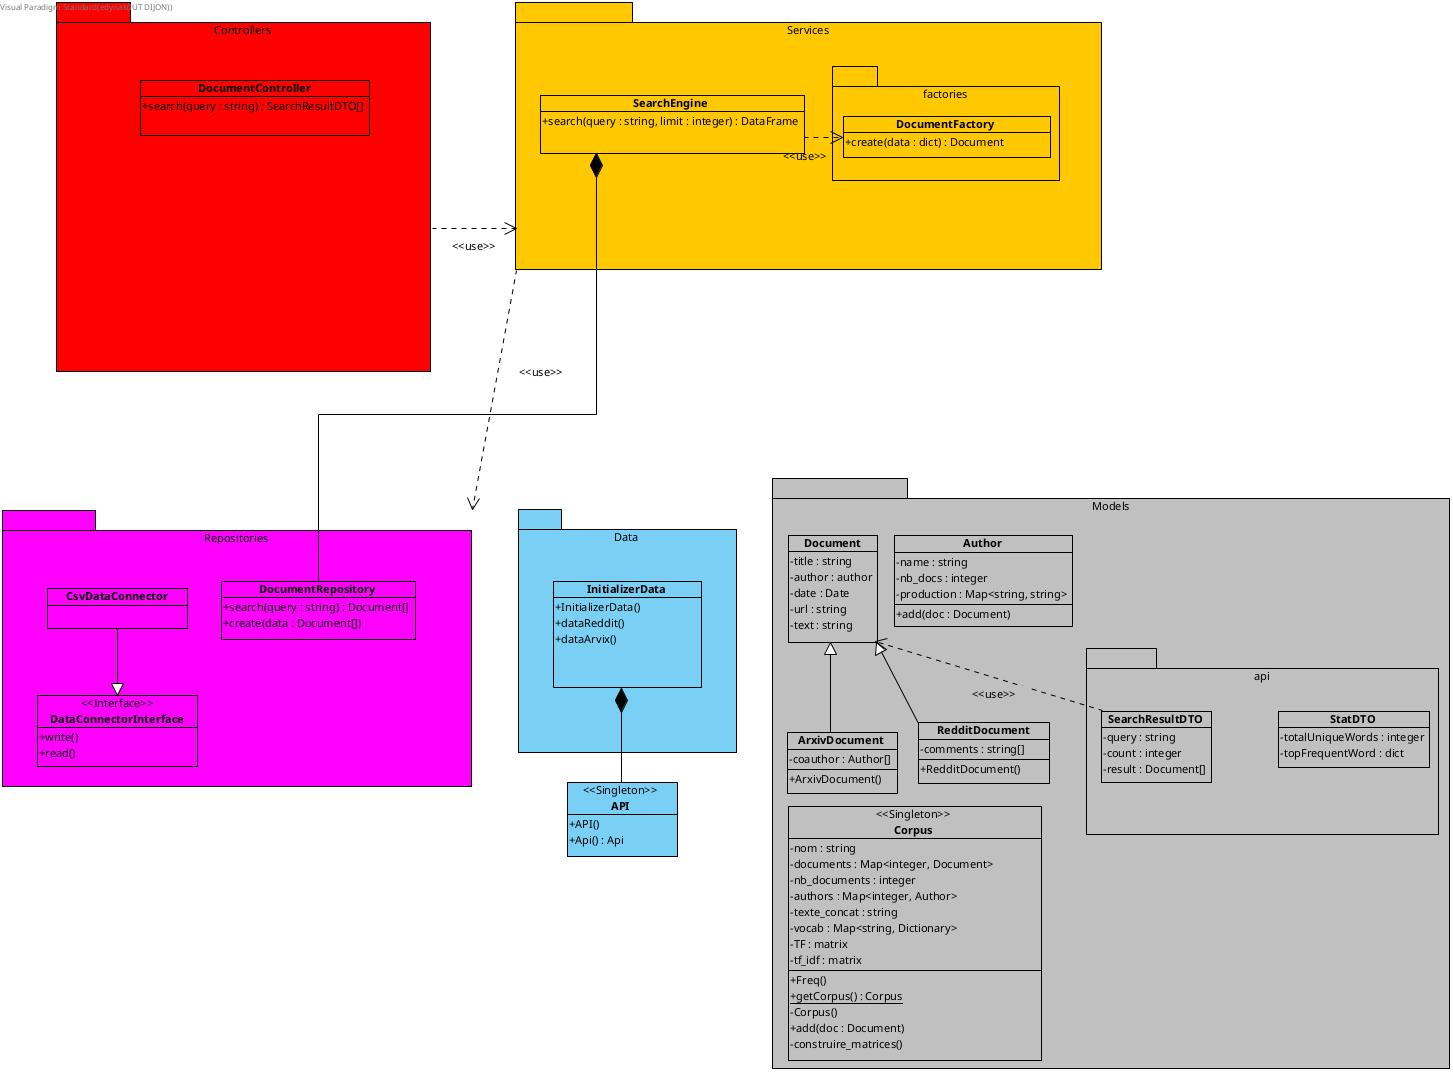
\includegraphics[width=15cm]{medias/archi}

\subsection{Organisation détaillée du front-end}

L'application front-end réside dans le répertoire \texttt{front/} et exploite les dernières avancées d'Angular (version 22) :
\begin{itemize}
    \item \textbf{Composants autonomes} : Suppression des modules complexes (\texttt{NgModule}) au profit de composants légers et indépendants.
    \item \textbf{Gestion d'état réactive par Signals} : Utilisation des primitives \texttt{signal}, \texttt{WritableSignal} et \texttt{computed} pour réagir aux flux de données sans surcharge de cycles de détection.
    \item \textbf{Intercepteur HTTP et indicateur de chargement} : L'intercepteur fonctionnel \texttt{httpInterceptorInterceptor} intercepte chaque requête sortante, incrémente le compteur du \texttt{LoaderService}, et le décrémente lors de la finalisation, permettant de connaitre l'état de chargement de l'application.
    \item \textbf{Composant partagé \texttt{SearchBar}} : Zone de saisie avec liaison bidirectionnelle (\texttt{[(ngModel)]}), capture des événements clavier (\textsc{Entrée}).
\end{itemize}

\subsection{Justification des choix technologiques et architecturaux}

\subsubsection{Pourquoi le patron Singleton ?}
La construction de l'index pour plusieurs milliers de documents représente un coût mémoire et processeur non négligeable. Si chaque requête HTTP devait réinstancier le \texttt{Corpus} ou recharger le fichier CSV, l'API s'effondrerait sous la charge. L'application du patron \textbf{Singleton} à la classe \texttt{Corpus} et à la classe \texttt{Api} garantit l'unicité de l'état en mémoire et partage la même structure d'indexation entre tous les appels concurrents.

\subsubsection{Pourquoi le patron Factory Method (\texttt{DocumentFactory}) ?}
Les données brutes lues depuis le fichier CSV contiennent un champ permettant de les différencier : \texttt{origin} (\texttt{"reddit"} ou \texttt{"arxiv"}). Confier l'instanciation directe au code consommateur créerait un couplage fort et multiplierait les blocs conditionnels. La \texttt{DocumentFactory} centralise la logique de construction et de désérialisation spécifique, garantissant l'extensibilité du code.

\subsubsection{Patron Repository et interface \texttt{DataConnectorInterface} ?}
L'accès au stockage local est isolé derrière l'interface abstraite \texttt{DataConnectorInterface}. Actuellement implémentée par \texttt{CsvDataConnector}, cette architecture permettrait de basculer sans aucun impact sur le reste de l'application vers un stockage SQLite, PostgreSQL ou MongoDB simplement en fournissant une nouvelle classe concrète.

\subsubsection{Pourquoi les Data Transfer Objects (DTO) ?}
Initialement, le moteur de recherche renvoyait directement des structures Pandas ou des dictionnaires non typés. L'introduction de \texttt{SearchResultDTO} et \texttt{StatDTO} a permis de stabiliser le contrat d'interface exposé au client Angular, protégeant le front-end contre toute modification de l'implémentation interne du back-end. En cas d'ajout de nouvelles fonctionnalités, il sera certes nécessaire de devoir modifier les objets DTOs, toutefois, ils permettent d'être certain d'obtenir les données attendues, ni plus ni moins.

\newpage

\subsection{Algorithmes spécifiques à l'application}

\subsubsection{Nettoyage et normalisation textuelle}
L'algorithme de prétraitement (\texttt{TextCleaner}) conditionne la qualité de l'indexation. Il applique les transformations successives :
\begin{enumerate}
    \item Passage intégral en minuscules pour éliminer la sensibilité à la casse.
    \item Remplacement systématique des sauts de ligne (\texttt{\textbackslash r\textbackslash n}, \texttt{\textbackslash n}) et tabulations par des espaces simples.
    \item Application d'une expression régulière de filtrage \texttt{[\^{}\textbackslash{}w\textbackslash{}s]|[\textbackslash{}d\_]} pour éliminer ponctuation, symboles spéciaux et chiffres.
    \item Réduction des espaces blancs contigus à une seule espace et suppression des espaces terminales (\textit{stripping}).
\end{enumerate}

\subsubsection{Construction du vocabulaire et calcul des fréquences}
La méthode \texttt{\_calculer\_frequences\_et\_vocabulaire()} parcourt chaque document du corpus :
\begin{itemize}
    \item Pour chaque mot $t$ d'un document $d$, la fréquence de terme globale $\text{TF}(t)$ est incrémentée.
    \item Un ensemble de mots uniques par document est conservé afin d'incrémenter la fréquence de document $\text{DF}(t)$ au plus une fois par document.
    \item Les termes sont triés par ordre alphabétique pour attribuer un identifiant unique de colonne.
\end{itemize}

\subsubsection{Schéma de pondération TF-IDF}
Pour chaque terme $t$ associé à sa colonne $j$, le poids IDF est calculé selon la formulation suivante :
\begin{equation}
    \text{IDF}(t) = \ln\left(\frac{1 + N}{1 + \text{DF}(t)}\right) + 1
\end{equation}
où $N$ désigne l'effectif global des documents dans le corpus. La matrice globale  $\mathbf{M}_{\text{TF-IDF}}$ est ensuite calculée par multiplication colonne à colonne :
\begin{equation}
    \mathbf{M}_{\text{TF-IDF}} = \mathbf{TF} \odot \vec{\text{IDF}}
\end{equation}

\newpage

\subsection{Problèmes rencontrés et solutions apportées}

\begin{enumerate}[leftmargin=*, label=\textbf{P\arabic*.}]
    \item \textbf{Instanciation répétée et bug de décorateur Singleton} :\\
    \textit{Problème} : La première implémentation du décorateur singleton stockait l'instance dans une liste globale mal réinitialisée, provoquant des erreurs lors des tests ou des exécutions imbriquées.\\
    \textit{Solution} : Refactorisation complète du décorateur avec un dictionnaire interne \texttt{instances} indexé par classe, garantissant une conservation sûre de l'instance unique.
    
    \item \textbf{Temps de recalcul de l'index vectoriel à l'ajout de documents} :\\
    \textit{Problème} : Reconstruire le vocabulaire et recalculer les matrices creuses à chaque ajout de document individuel pénalisait les temps de réponse de manière inacceptable.\\
    \textit{Solution} : Implémentation du patron de chargement paresseux (\textit{Lazy Loading}) via des \texttt{@property} avec mise en cache. Les calculs ne sont déclenchés que lors du premier accès en lecture. L'ajout d'un document réinitialise simplement les caches à \texttt{None}.

    \item \textbf{Épuisement des quotas d'appels API et dépendance réseau} :\\
    \textit{Problème} : Interroger les API Reddit et arXiv à chaque lancement de l'application engendrait une forte latence et risquait d'induire un blocage IP pour requêtes excessives.\\
    \textit{Solution} : La classe \texttt{InitializerData} vérifie au préalable si le fichier \texttt{data.csv} existe et contient des données exploitables. La collecte distante n'est exécutée qu'en cas d'absence complète de données locales.

    \item \textbf{Blocage CORS entre le client Angular et le serveur FastAPI} :\\
    \textit{Problème} : En phase d'intégration du front-end, le navigateur bloquait les requêtes émises depuis l'origine \texttt{http://localhost:4200} vers l'API sur \texttt{http://localhost:8000}.\\
    \textit{Solution} : Intégration du middleware \texttt{CORSMiddleware} dans FastAPI, autorisant explicitement les requêtes en provenance de \texttt{http://localhost:4200} avec les méthodes et en-têtes nécessaires.

    \item \textbf{Organisation confuse lors du passage au Front-end} :\\
    \textit{Problème} : La racine du projet mélangeait scripts Python, fichiers de dépendances et configuration globale, ce qui rendait impossible l'installation propre d'une application Angular.\\
    \textit{Solution} : Restructuration complète du dépôt sous forme de mono-repo, délimitant strictement les dossiers \texttt{back/} (Python, FastAPI, dépendances pip) et \texttt{front/} (TypeScript, Angular, node\_modules).
\end{enumerate}

\newpage

\subsection{Exemple commenté d'utilisation du programme}

Voici le scénario complet d'une session de recherche standard :

\begin{enumerate}
    \item \textbf{Amorçage du serveur d'application} :
        \begin{verbatim}
$ cd back/
$ fastapi dev main.py
        \end{verbatim}
        Le composant \texttt{Api} est instancié. \texttt{InitializerData} valide l'intégrité de \texttt{data.csv}. \texttt{CsvDataConnector} lit les enregistrements et \texttt{DocumentFactory} peuple le singleton \texttt{Corpus}. L'API démarre sur \url{http://127.0.0.1:8000} (ou \url{http://localhost:8000}).

    \item \textbf{Lancement de l'interface utilisateur} :
        \begin{verbatim}
$ cd front/
$ npm start
        \end{verbatim}
        Le serveur de développement Angular compile l'application et sert l'interface sur \texttt{http://localhost:4200}.

    \item \textbf{Navigation et saisie de la requête} :
        L'utilisateur se rend sur \url{http://127.0.0.1:4200} (ou \url{http://localhost:4200}). La page d'accueil affiche la barre de recherche. L'utilisateur renseigne les termes «\texttt{reinforcement learning robotics}» et valide avec la touche \textsc{Entrée}.

    \item \textbf{Traitement et transition dans l'application} :
        Le composant \texttt{SearchBar} déclenche la navigation vers \texttt{/search?query=reinforcement+learning+robotics}. La page \texttt{SearchingPage} est activée. Elle sollicite \texttt{SearchService.search()}, qui émet la requête HTTP correspondante.
        L'intercepteur HTTP active le signal d'état de chargement dans \texttt{LoaderService}.

\newpage
    \item \textbf{Résolution sur le serveur} :
        Le contrôleur \texttt{SearchEngineController} reçoit la requête, la transmet au \texttt{SearchEngine}. Ce dernier nettoie la chaîne, calcule le produit scalaire sur la matrice creuse TF-IDF et classe les meilleurs documents. Le contrôleur renvoie un objet \texttt{SearchResultDTO} sérialisé en JSON :
        \begin{verbatim}
{
  "query": "reinforcement learning robotics",
  "count": 10,
  "result": [
    {
      "id": 112,
      "score": 0.7421,
      "titre": "Deep Reinforcement Learning for Robot Navigation",
      "origine": "arxiv",
      "url": "http://arxiv.org/abs/2103.xxxxx",
      "auteur": "Smith et al.",
      "texte": "This paper presents a novel model-free RL algorithm..."
    }
  ]
}
        \end{verbatim}

    \item \textbf{Affichage et exploitation du résultat} :
        Le flux HTTP se clôture, le \texttt{LoaderService} rétablit l'affichage normal. La directive structurelle \texttt{@for} restitue les cartes des dix documents les plus pertinents, avec leur score, leur titre cliquable ouvrant la source originale (arXiv ou Reddit) et un extrait représentatif de leur contenu.
\end{enumerate}

\newpage

\section{Étapes de réflexion et de réalisation}

\subsection{Fondations orientées objet et collecte multi-sources (Branche part-1)}

\subsubsection{10 et 15 septembre 2026}
Poser les bases d'un environnement de travail propre. Mise en place du fichier \texttt{.gitignore} pour exclure les fichiers d'environnement Python ou de cache.

\subsubsection{17 septembre 2026}
\begin{itemize}
    \item Une classe abstraite de base \texttt{Document} regroupant les propriétés : titre, auteur, date, url, texte.
    \item Des sous-classes spécialisées (\texttt{RedditDocument}, \texttt{ArvixDocument}) enrichies d'autres attributs ajoutés dans leur source d'origine.
    \item La classe \texttt{Corpus} agissant comme conteneur des documents.
    \item Une première abstraction de persistance avec l'interface \texttt{DataConnectorInterface} et son implémentation \texttt{CsvDataConnector}.
    \item Une première tentative de mise en œuvre du patron \texttt{Singleton}.
\end{itemize}

\subsubsection{07 octobre 2026}
\begin{itemize}
    \item Intégration du framework \textbf{FastAPI} et du serveur \textbf{Uvicorn}.
    \item Découplage de la couche d'exposition via une interface \texttt{IController} et un contrôleur dédié \texttt{SearchEngineController}.
    \item Création de l'entité \texttt{Api} pour encapsuler l'application web.
\end{itemize}

\subsubsection{08 octobre 2026}
\begin{itemize}
    \item Implémentation effective de l'extraction sur ArXiv et sur Reddit.
    \item Conception d'un mécanisme de cache local vérifiant si \texttt{data.csv} est déjà alimenté avant d'effectuer de nouveaux appels réseau.
    \item Correction du décorateur \texttt{Singleton} devenu parfaitement fiable.
    \item Introduction du patron \textbf{Factory Method} (\texttt{DocumentFactory}) permettant d'isoler l'analyse du champ  \texttt{origin} et d'instancier la classe concrète adaptée.
\end{itemize}

\subsection{Mathématisation vectorielle et moteur de recherche (Branche part-2)}

\subsubsection{02 novembre 2026}

\begin{itemize}
	\item Introduction du module autonome \texttt{TextCleaner} avec sa méthode \texttt{nettoyer\_texte}.
	\item Implémentation du concordancier par expressions régulières (\texttt{Corpus.concorde}).
	\item Dérivation du vocabulaire global et calcul des fréquences globales (TF) et documentaires (DF).
\end{itemize}

Implémentation complète de \texttt{SearchEngine} :
\begin{itemize}
	\item Vectorisation à la volée de la requête utilisateur sur la base du vocabulaire indexé et des coefficients IDF.
	\item Calcul vectorisé de la similarité cosinus par produit matriciel creux.
	\item Extraction des $n$ meilleurs scores et enrichissement des résultats avec métadonnées complètes.
\end{itemize}

\begin{itemize}
	\item Exposition des deux routes REST principales : \texttt{/search} et \texttt{/stats}.
\end{itemize}



\newpage

\subsection{Interface moderne Angular et refactorisation mono-repo}

\subsubsection{06 novembre 2026}
\begin{itemize}
    \item Choix de développer un front-end complet en \textbf{Angular 22} (\textit{Single Page Application}).
    \item Réorganisation du dépôt en \textbf{mono-repo} séparé en deux dossiers hermétiques : \texttt{back/} et \texttt{front/}.
    \item Introduction des DTOs (\texttt{SearchResultDTO}, \texttt{StatDTO}) pour séparer le modèle interne de calcul du schéma JSON envoyé au client.
    \item Sécurisation des flux inter-domaines par l'ajout de \texttt{CORSMiddleware} dans FastAPI autorisant \texttt{http://localhost:4200}.
    \item Conception d'une interface responsive avec gestion d'état réactive (Angular Signals) et intercepteur HTTP pour le retour visuel de chargement.
\end{itemize}

\newpage

\section{La validation}

\subsection{Procédures de tests unitaires}

\subsubsection{Tests unitaires du back-end Python}
Les méthodes critiques du back-end ont fait l'objet de vérifications unitaires ciblées :
\begin{itemize}
    \item \textbf{Validation du nettoyage textuel (\texttt{TextCleaner})} : Vérification de la suppression des caractères accentués parasites, des tabulations, des retours chariot multiples et de la conservation des mots-clés.
    \item \textbf{Validation de la fabrique (\texttt{DocumentFactory})} : Contrôle de l'instanciation d'un \texttt{RedditDocument} lorsque \texttt{origin == "reddit"} et d'un \texttt{ArvixDocument} lorsque \texttt{origin == "arxiv"}.
    \item \textbf{Validation du calcul matriciel} : Vérification que la matrice TF-IDF produite a les bonnes dimensions et que ses éléments sont strictement non négatifs.
    \item \textbf{Validation interactive des endpoints FastAPI} : Utilisation de l'interface Swagger générée sur \url{http://localhost:8000/docs} pour éprouver les codes d'état HTTP et la conformité des schémas JSON retournés.
\end{itemize}

\subsection{Tests globaux via l'interface utilisateur}

\begin{table}[H]
	\centering
	\caption{Cahier de recette et validation des tests globaux de l'interface utilisateur}
	\label{tab:tests_globaux}
	\begin{singlespace}
	\renewcommand{\arraystretch}{1.1}
	\small
	\begin{tabularx}{\linewidth}{>{\bfseries}p{2.8cm} p{2.8cm} X c}
		\toprule
		\textbf{Scénario de test} & \textbf{Données d'entrée} & \textbf{Comportement attendu et vérifications} & \textbf{Résultat} \\
		\midrule
		Recherche nominale simple & \texttt{"neural"} & Interception de la saisie, appel à \texttt{/search?query=neural}, affichage des 10 documents les plus pertinents avec titres, liens et extraits. & \textcolor{OliveGreen}{\textbf{Conforme}} \\
		Recherche composite multi-termes & \texttt{"deep learning vision"} & Vectorisation conjointe, classement privilégiant les documents maximisant la similarité cosinus avec l'ensemble des termes. & \textcolor{OliveGreen}{\textbf{Conforme}} \\
		Insensibilité à la casse & \texttt{"MaChiNe LeArNiNg"} & Normalisation automatique par \texttt{TextCleaner} ; résultats et scores strictement identiques à \texttt{"machine learning"}. & \textcolor{OliveGreen}{\textbf{Conforme}} \\
		Tolérance aux bruits et ponctuation & \texttt{"AI \& robotics!?\#"} & Épuration des caractères non alphanumériques superflus ; recherche traitée comme équivalente à \texttt{"ai robotics"}. & \textcolor{OliveGreen}{\textbf{Conforme}} \\
		Requête vide ou espaces & \texttt{""} ou \texttt{"\quad"} & Blocage de la soumission au niveau du composant \texttt{SearchBar} ; aucune navigation superflue ni appel réseau déclenché. & \textcolor{OliveGreen}{\textbf{Conforme}} \\
		Termes hors vocabulaire & \texttt{"unknown123"} & Similarité cosinus nulle sur tout le corpus ; déclenchement du bloc \texttt{@empty} avec message convivial invitant à retenter. & \textcolor{OliveGreen}{\textbf{Conforme}} \\
		Indicateur de chargement réactif & Requête réseau & Activation synchrone du \texttt{LoaderService} via l'intercepteur HTTP ; masquage temporaire des résultats et affichage du spinner. & \textcolor{OliveGreen}{\textbf{Conforme}} \\
		Consultation des sources externes & Clic sur un titre de résultat & Exploitation du champ discriminant \texttt{url} pour rediriger l'utilisateur vers la publication d'origine (arXiv ou Reddit). & \textcolor{OliveGreen}{\textbf{Conforme}} \\
		Recherche consécutive directe & Nouvelle saisie depuis la page & Mise à jour réactive du paramètre d'URL \texttt{?query=...} via le routeur Angular ; rafraîchissement immédiat de la liste de résultats. & \textcolor{OliveGreen}{\textbf{Conforme}} \\
		\bottomrule
	\end{tabularx}
	\end{singlespace}
\end{table}

\newpage

\section{La maintenance et les perspectives d'évolution}

\subsection{Évolutions fonctionnelles envisageables}

\subsubsection{Intégration de nouvelles sources documentaires (ex. HAL, Wikipedia)}
\begin{itemize}
    \item \textbf{Mise en place} : Créer une sous-classe \texttt{HalDocument} étendant \texttt{Document}, ajouter une méthode de collecte dans \texttt{InitializerData}, et déclarer le cas d'instanciation correspondant dans la \texttt{DocumentFactory}.
    \item \textbf{Evaluation de faisabilité : Facile}. Grâce au patron Factory et à l'architecture ouverte de la hiérarchie de classes, aucune modification des algorithmes d'indexation ou des contrôleurs n'est requise.
\end{itemize}

\subsubsection{Filtrage multicritère (par date, source ou auteur)}
\begin{itemize}
    \item \textbf{Mise en place} : Étendre les paramètres de l'endpoint \texttt{/search} dans \texttt{SearchEngineController} avec des options optionnelles (\texttt{origin}, \texttt{author}, \texttt{date\_from}) et appliquer un masque de filtrage vectoriel sur le tableau de résultats final.
    \item \textbf{Evaluation de faisabilité : Facile à Moyenne}. Les métadonnées sont déjà conservées dans le conteneur \texttt{Corpus} et retournées dans les résultats.
\end{itemize}

\subsubsection{Pagination des résultats}
\begin{itemize}
    \item \textbf{Mise en place} : Ajouter un paramètre \texttt{page} et \texttt{page\_size} sur l'API, et utiliser l'opérateur de slicing sur le vecteur ordonné des indices retournés par \texttt{numpy.argsort}.
    \item \textbf{Evaluation de faisabilité : Très facile}.
\end{itemize}

\subsection{Amélioration de l'IHM}
\begin{itemize}
	\item \textbf{Mise en place} : Créer une charte graphique au site, un logo, permettant de rendre cela plus agréable
	\item \textbf{Evaluation de faisabilité : Facile à Difficile}. Tout dépend des modifications qui sont apportées à l'application, jusqu'où on développe la charte graphique, etc...
\end{itemize}

\newpage

\subsection{Évolutions techniques envisageables}

\subsubsection{Ajout d'autres thèmes de recherche}
\begin{itemize}
    \item \textbf{Mise en place} : Ajouter d'autres mots clés de recherche lors de la récupération des données via les APIs.
    \item \textbf{Evaluation de faisabilité : Haute}. Facilement mis en place pour plusieurs thèmes, toutefois si le nombre de thèmes est trop grand, risque de baisse de performances du moteur lié à la volumétrie de données dans un format de stockage inadapté à celle-ci.
\end{itemize}

\subsubsection{Remplacement de la méthode de stockage de données}
\begin{itemize}
	\item \textbf{Mise en place} : Transformer notre base de données actuelle (fichier csv) en une vraie base de données, ayant de meilleurs performances sur la récupération des données, et notamment pour les tris de données
	\item \textbf{Evaluation de faisabilité : Moyenne}. D'un point de vue, la mise en place est plutôt rapide car il suffit uniquement d'adapter notre implémentation de l'interface \texttt{DataConnectorInterface} avec une base de données. Toutefois, côté base de données, il faut recréer les schémas correspondants, bien structuré les tables afin que celle-ci aient un temps de réponse correct, et cela peut prendre un certain temps et une certaine complexité.
\end{itemize}

\newpage

\section{Utilisation de l'IA}

Dans ce projet, l'IA a été utilisé pour les éléments suivants :

\begin{enumerate}
	\item \textbf{Aide dans la mise en place architecturale de l'API en Python} : n'ayant jamais utilisé FastAPI comme librairie, mais souhaitant imposé une architecture maitrisée (Controllers -> Service -> Repository), l'IA m'a permis de mieux structurer mon code pour la suite.
	\item \textbf{Aide à la mise en place du rapport :} Aide pour la récupération des différents tests / commits depuis le dépôt Git, et aide pour l'utilisation de LaTeX. N'ayant jamais utilisé également cette méthode de création de documents, et ayant connaissance qu'il sera utile dans d'autres matières ainsi que dans le monde de la recherche, celui-ci a permis de créer rapidement la structure du document.
	\item \textbf{Vérification de la qualité du code} : Régulièrement durant le processus, je demandais à ce que l'IA vérifie la qualité afin que celle-ci ne se détériore pas trop.
	\item \textbf{Lors d'un blocage après de multiples essais} : Lorsque le code ne fonctionnait pas, notamment dans les notions mathématiques, j'ai quelques fois demandé à l'IA d'analyser le code fait (qui ne marchait pas) et d'expliquer pourquoi cela ne fonctionne pas, que cela soit d'un point de vue code ou purement mathématiques. L'objectif n'étant pas de faire à ma place, mais de comprendre mes erreurs et de pouvoir les remédier.

\end{enumerate}

\newpage

\section{Conclusion}

Ce projet a concrétisé la mise en œuvre d'un moteur de recherche textuel complet, rigoureux et performant. En partant d'un cahier des charges exigeant, le travail a couvert l'ensemble du cycle de vie d'une application logicielle moderne :
\begin{enumerate}
    \item L'\textbf{analyse approfondie du problème} et l'identification des entités et abstractions clés ;
    \item La \textbf{conception orientée objet} mobilisant des patrons éprouvés (Singleton, Factory, Repository, DTO, Lazy Loading) ;
    \item L'\textbf{ingénierie mathématique et algorithmique}, conjuguant normalisation textuelle, pondération TF-IDF et calcul matriciel creux ultra-performant sous SciPy ;
    \item Le \textbf{développement d'une interface web moderne et réactive} en Angular 22, découplée du back-end par une API REST conforme aux standards de l'art ;
    \item Une \textbf{stratégie de validation rigoureuse} unissant tests unitaires et tests fonctionnels d'intégration.
\end{enumerate}

L'application constitue aujourd'hui un socle solide, documenté et immédiatement extensible vers de nouveaux horizons technologiques.


\end{document}
